% CORRELATION
\subsection{Correlation}
\label{subsection:corr}
The application of a linear filter $h(u,v)$ to an image $f(i,j)$ may be described as follows

\begin{equation} \label{eq:1}
g(i,j) = \sum_{u=-k}^{k}\sum_{v = -l}^{l}f(i+u,j+v)h(u,v)
\end{equation}

$g(i,j)$ is the output image. Performing correlation with a filter may be notated more concisely by the correlation operator.

\[g = f \otimes h\]

Correlation measures the \emph{similarity} between two signals and as both digital images and linear filters are two dimensional signals by correlating them we can see where they are most similar. Performing correlation between them will produce an output image whose highest values correspond to where the image and filter were most similar \cite{optimalKernel}. This is an important operation in image classification as it can be used to highlight features in an image and diminish everything else by correlating a filter that describes the desired feature. The feature could be as simple as a straight line as in a Sobel filter (Figure \ref{fig:sobel_filters}) or as specific as the outline of a car wheel. This method of feature detection is called \emph{templating}.

In Figure \ref{fig:sobel_apply} vertical and horizontal Sobel filters are applied to produce images that emphasise lines that match the orientation in the respective filter, the lines that are most similar. The result is black and white as the initial output image's intensities have been thresholded to either be 1 or 0. I.e. where initial output image is $F(x,y) = z$ and $T$ is the threshold intensity:

\begin{equation}
  Binary Output = 
  \begin{cases}
    1 & \text{if $z$ $>=$ $T$} \\
    0 & \text{if $z$ $<$  $T$}
  \end{cases}
  \label{eq:threshold}
\end{equation}

% SOBEL MASKS
\begin{figure}[H]
  \begin{subfigure}[b]{0.49\textwidth}
    \[
    \begin{bmatrix*}[l]
     -1 & -1 & -1 \\
      \phantom{-}2 & \phantom{-}2 & \phantom{-}2 \\
      -1 & -1 & -1 
    \end{bmatrix*}
    \]
    \caption{Horizontal Sobel Filter Mask}
    \label{rfidtest_xaxis}
\end{subfigure}
\begin{subfigure}[b]{0.49\textwidth}
  \[ 
    \begin{bmatrix}
      -1 & 2 & -1 \\
      -1 & 2 & -1 \\
      -1 & 2 & -1
    \end{bmatrix}
    \]
    \caption{Vertical Sobel Filter Mask}  
\end{subfigure}
    \caption{Sobel Filters}
    \label{fig:sobel_filters}
\end{figure}

% SOBEL FILTER APPLICATION
\begin{figure}[H]
  \centering
  \begin{subfigure}[b]{0.3\textwidth}
      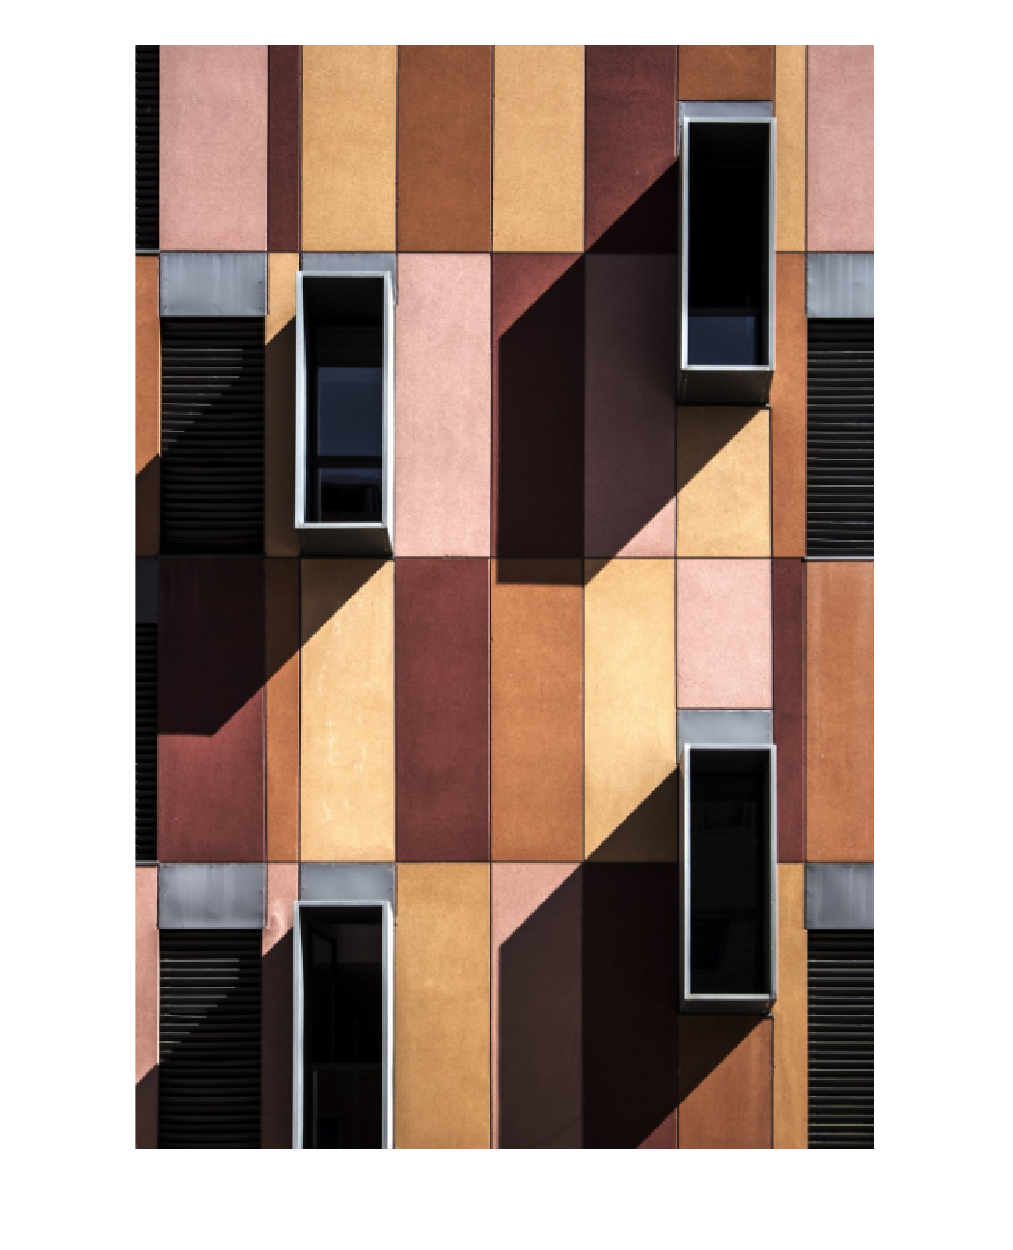
\includegraphics[width=\textwidth]{im_color}
      \caption{Image by Simone Hutsch}
  \end{subfigure}
  \begin{subfigure}[b]{0.3\textwidth}
      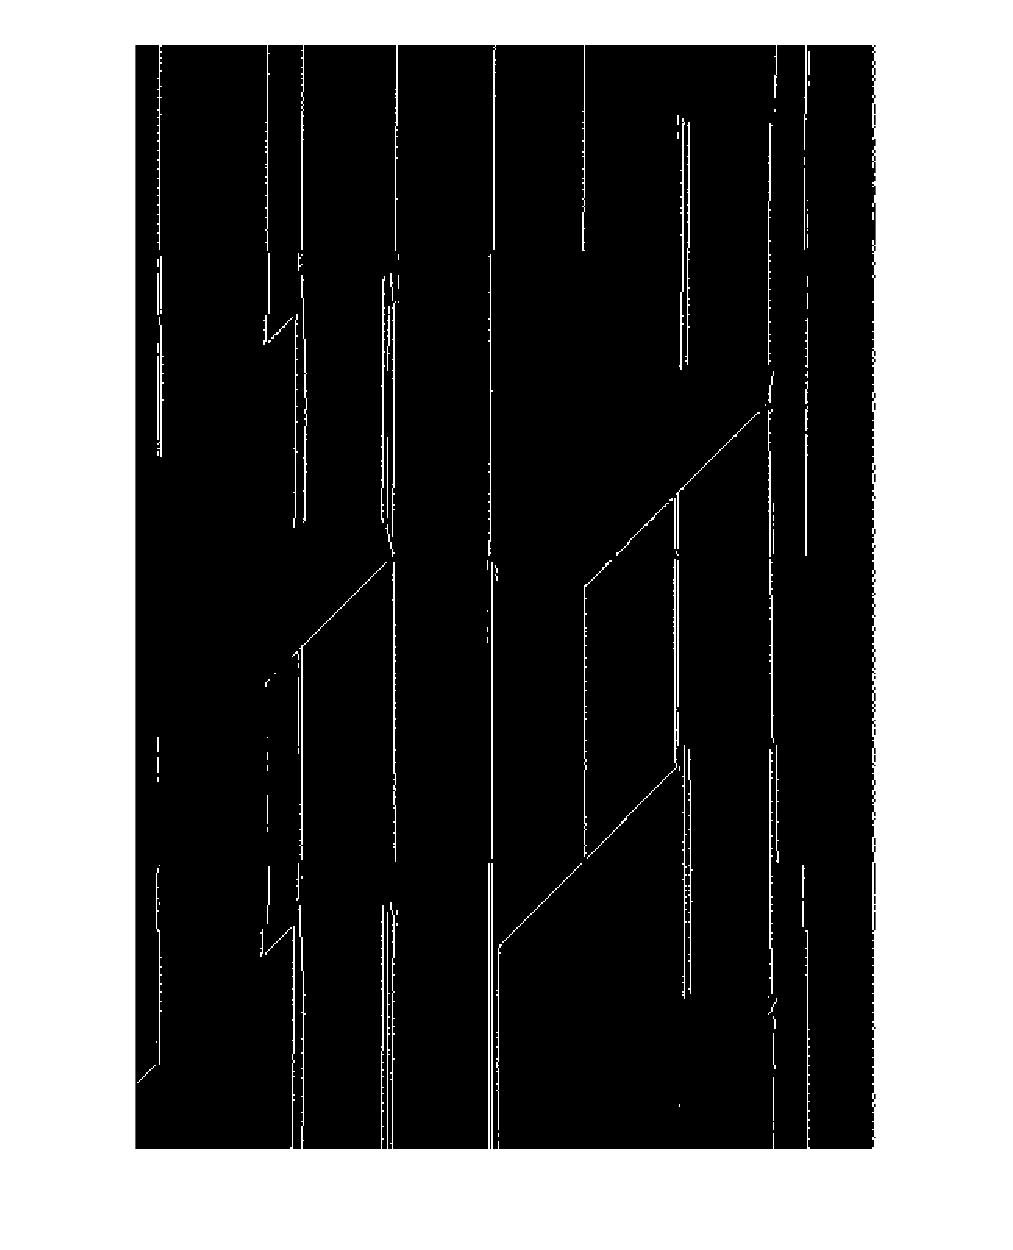
\includegraphics[width=\textwidth]{gv}
      \caption{Vertical Sobel Filter}
      \label{fig:vert}
  \end{subfigure}
  \begin{subfigure}[b]{0.3\textwidth}
      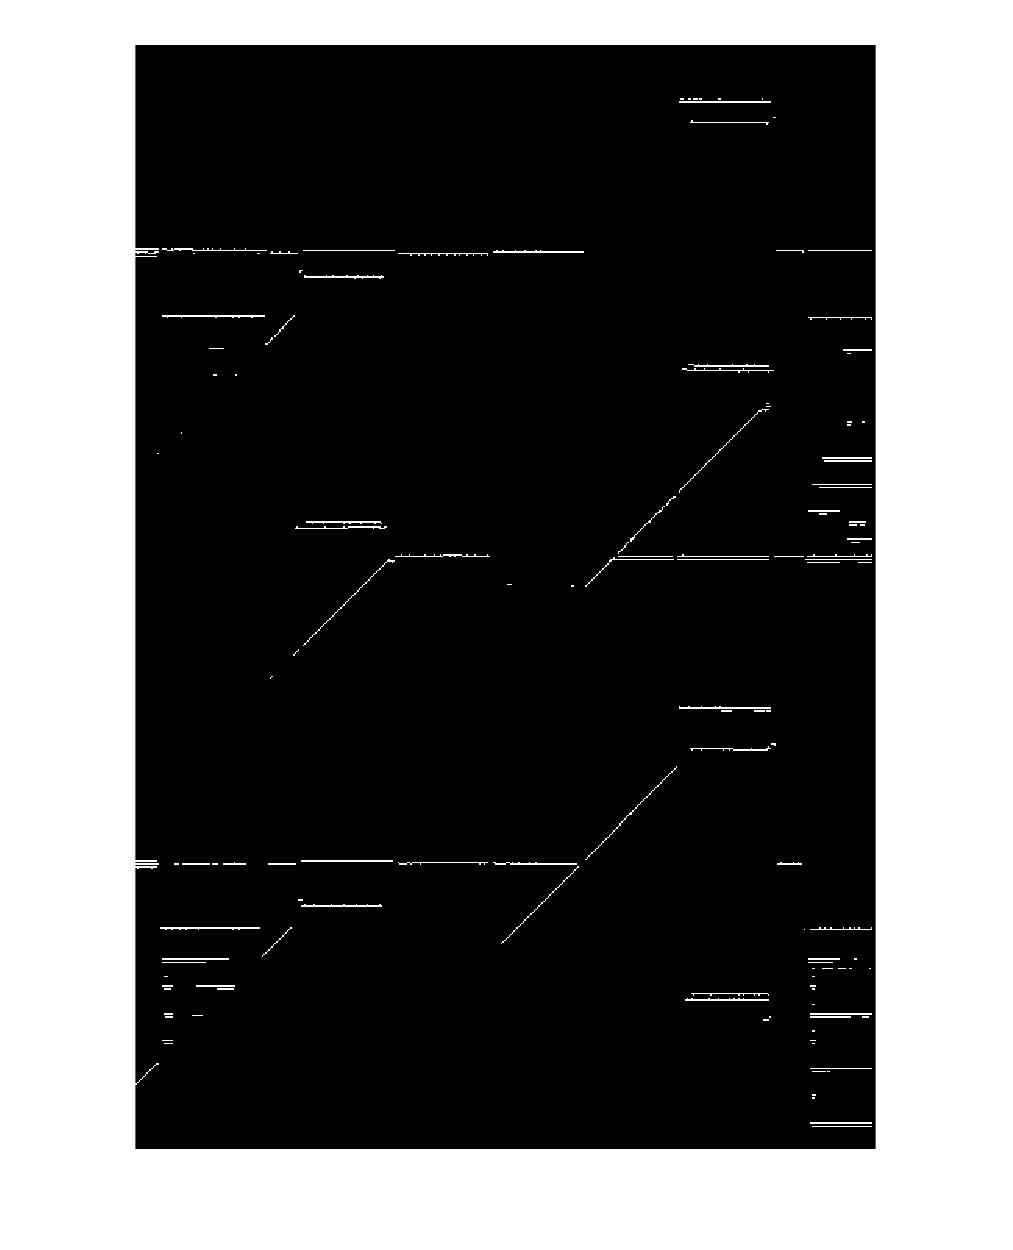
\includegraphics[width=\textwidth]{gh}
      \caption{Horizontal Sobel Filter}
      \label{fig:hoz}
  \end{subfigure}
  \caption{Application of Sobel filters to exagerate lines.}
  \label{fig:sobel_apply}
\end{figure}

Correlation is \emph{shift invariant}, which means that it does the same thing no matter where in an image it is applied. To satisfy this property correlation may be superpositioned 

\[a(f_1 + f_2) = af_1 + af_2\]

and abides by the shift invariance principle

\[g(i,j)=f(i+k,j+l) \Leftrightarrow\ (h\circ g)(i,j)=(h\circ f)(i+k,j+l)\]

Correlation has the side effect of flipping both horizontally and vertically the location of output points relative to the center point (\emph{reference point}) in the original image which may be undesirable as can be observed in Figure \ref{fig:correlation}.

% CORRELATION EXAMPLE  %
\begin{figure}[H] 
  \centering
  \begin{tabular}{ccccc}
      \begin{tabular}{|c|c|c|c|c|}
      \hline
      0 & 0 & 0 & 0 & 0 \\[1pt]
      \hline
      0 & 0 & 0 & 0 & 0 \\[1pt]
      \hline
      0 & 0 & 1 & 0 & 0 \\[1pt]
      \hline
      0 & 0 & 0 & 0 & 0 \\[1pt]
      \hline
      0 & 0 & 0 & 0 & 0 \\[1pt]
      \hline
      \end{tabular}%
    & $\otimes$ &
    \begin{tabular}{|c|c|c|}
      \hline
      a & b & c \\
      \hline
      d & e & f \\
      \hline
      g & h & i \\
      \hline 
    \end{tabular}
    & $=$ &
    \begin{tabular}{|c|c|c|c|c|}
      \hline
      0 & 0 & 0 & 0 & 0 \\[1pt]
      \hline
      0 & \textbf{i} & \textbf{h} & \textbf{g} & 0 \\[1pt]
      \hline
      0 & \textbf{f} & \textbf{e} & \textbf{d} & 0 \\[1pt]
      \hline
      0 & \textbf{c} & \textbf{b} & \textbf{a} & 0 \\[1pt]
      \hline
      0 & 0 & 0 & 0 & 0 \\[1pt]
      \hline
    \end{tabular} \\
    $F(x,y)$ & & $H(u,v)$& & $G(x,y)$ \\
  \end{tabular}
  \caption{Correlation of a filter and an image.}
  \label{fig:correlation}
\end{figure}